\documentclass[1p]{elsarticle_modified}
%\bibliographystyle{elsarticle-num}

%\usepackage[colorlinks]{hyperref}
%\usepackage{abbrmath_seonhwa} %\Abb, \Ascr, \Acal ,\Abf, \Afrak
\usepackage{amsfonts}
\usepackage{amssymb}
\usepackage{amsmath}
\usepackage{amsthm}
\usepackage{scalefnt}
\usepackage{amsbsy}
\usepackage{kotex}
\usepackage{caption}
\usepackage{subfig}
\usepackage{color}
\usepackage{graphicx}
\usepackage{xcolor} %% white, black, red, green, blue, cyan, magenta, yellow
\usepackage{float}
\usepackage{setspace}
\usepackage{hyperref}

\usepackage{tikz}
\usetikzlibrary{arrows}

\usepackage{multirow}
\usepackage{array} % fixed length table
\usepackage{hhline}

%%%%%%%%%%%%%%%%%%%%%
\makeatletter
\renewcommand*\env@matrix[1][\arraystretch]{%
	\edef\arraystretch{#1}%
	\hskip -\arraycolsep
	\let\@ifnextchar\new@ifnextchar
	\array{*\c@MaxMatrixCols c}}
\makeatother %https://tex.stackexchange.com/questions/14071/how-can-i-increase-the-line-spacing-in-a-matrix
%%%%%%%%%%%%%%%

\usepackage[normalem]{ulem}

\newcommand{\msout}[1]{\ifmmode\text{\sout{\ensuremath{#1}}}\else\sout{#1}\fi}
%SOURCE: \msout is \stkout macro in https://tex.stackexchange.com/questions/20609/strikeout-in-math-mode

\newcommand{\cancel}[1]{
	\ifmmode
	{\color{red}\msout{#1}}
	\else
	{\color{red}\sout{#1}}
	\fi
}

\newcommand{\add}[1]{
	{\color{blue}\uwave{#1}}
}

\newcommand{\replace}[2]{
	\ifmmode
	{\color{red}\msout{#1}}{\color{blue}\uwave{#2}}
	\else
	{\color{red}\sout{#1}}{\color{blue}\uwave{#2}}
	\fi
}

\newcommand{\Sol}{\mathcal{S}} %segment
\newcommand{\D}{D} %diagram
\newcommand{\A}{\mathcal{A}} %arc


%%%%%%%%%%%%%%%%%%%%%%%%%%%%%5 test

\def\sl{\operatorname{\textup{SL}}(2,\Cbb)}
\def\psl{\operatorname{\textup{PSL}}(2,\Cbb)}
\def\quan{\mkern 1mu \triangleright \mkern 1mu}

\theoremstyle{definition}
\newtheorem{thm}{Theorem}[section]
\newtheorem{prop}[thm]{Proposition}
\newtheorem{lem}[thm]{Lemma}
\newtheorem{ques}[thm]{Question}
\newtheorem{cor}[thm]{Corollary}
\newtheorem{defn}[thm]{Definition}
\newtheorem{exam}[thm]{Example}
\newtheorem{rmk}[thm]{Remark}
\newtheorem{alg}[thm]{Algorithm}

\newcommand{\I}{\sqrt{-1}}
\begin{document}

%\begin{frontmatter}
%
%\title{Boundary parabolic representations of knots up to 8 crossings}
%
%%% Group authors per affiliation:
%\author{Yunhi Cho} 
%\address{Department of Mathematics, University of Seoul, Seoul, Korea}
%\ead{yhcho@uos.ac.kr}
%
%
%\author{Seonhwa Kim} %\fnref{s_kim}}
%\address{Center for Geometry and Physics, Institute for Basic Science, Pohang, 37673, Korea}
%\ead{ryeona17@ibs.re.kr}
%
%\author{Hyuk Kim}
%\address{Department of Mathematical Sciences, Seoul National University, Seoul 08826, Korea}
%\ead{hyukkim@snu.ac.kr}
%
%\author{Seokbeom Yoon}
%\address{Department of Mathematical Sciences, Seoul National University, Seoul, 08826,  Korea}
%\ead{sbyoon15@snu.ac.kr}
%
%\begin{abstract}
%We find all boundary parabolic representation of knots up to 8 crossings.
%
%\end{abstract}
%\begin{keyword}
%    \MSC[2010] 57M25 
%\end{keyword}
%
%\end{frontmatter}

%\linenumbers
%\tableofcontents
%
\newcommand\colored[1]{\textcolor{white}{\rule[-0.35ex]{0.8em}{1.4ex}}\kern-0.8em\color{red} #1}%
%\newcommand\colored[1]{\textcolor{white}{ #1}\kern-2.17ex	\textcolor{white}{ #1}\kern-1.81ex	\textcolor{white}{ #1}\kern-2.15ex\color{red}#1	}

{\Large $\underline{12a_{0972}~(K12a_{0972})}$}

\setlength{\tabcolsep}{10pt}
\renewcommand{\arraystretch}{1.6}
\vspace{1cm}\begin{tabular}{m{100pt}>{\centering\arraybackslash}m{274pt}}
\multirow{5}{120pt}{
	\centering
	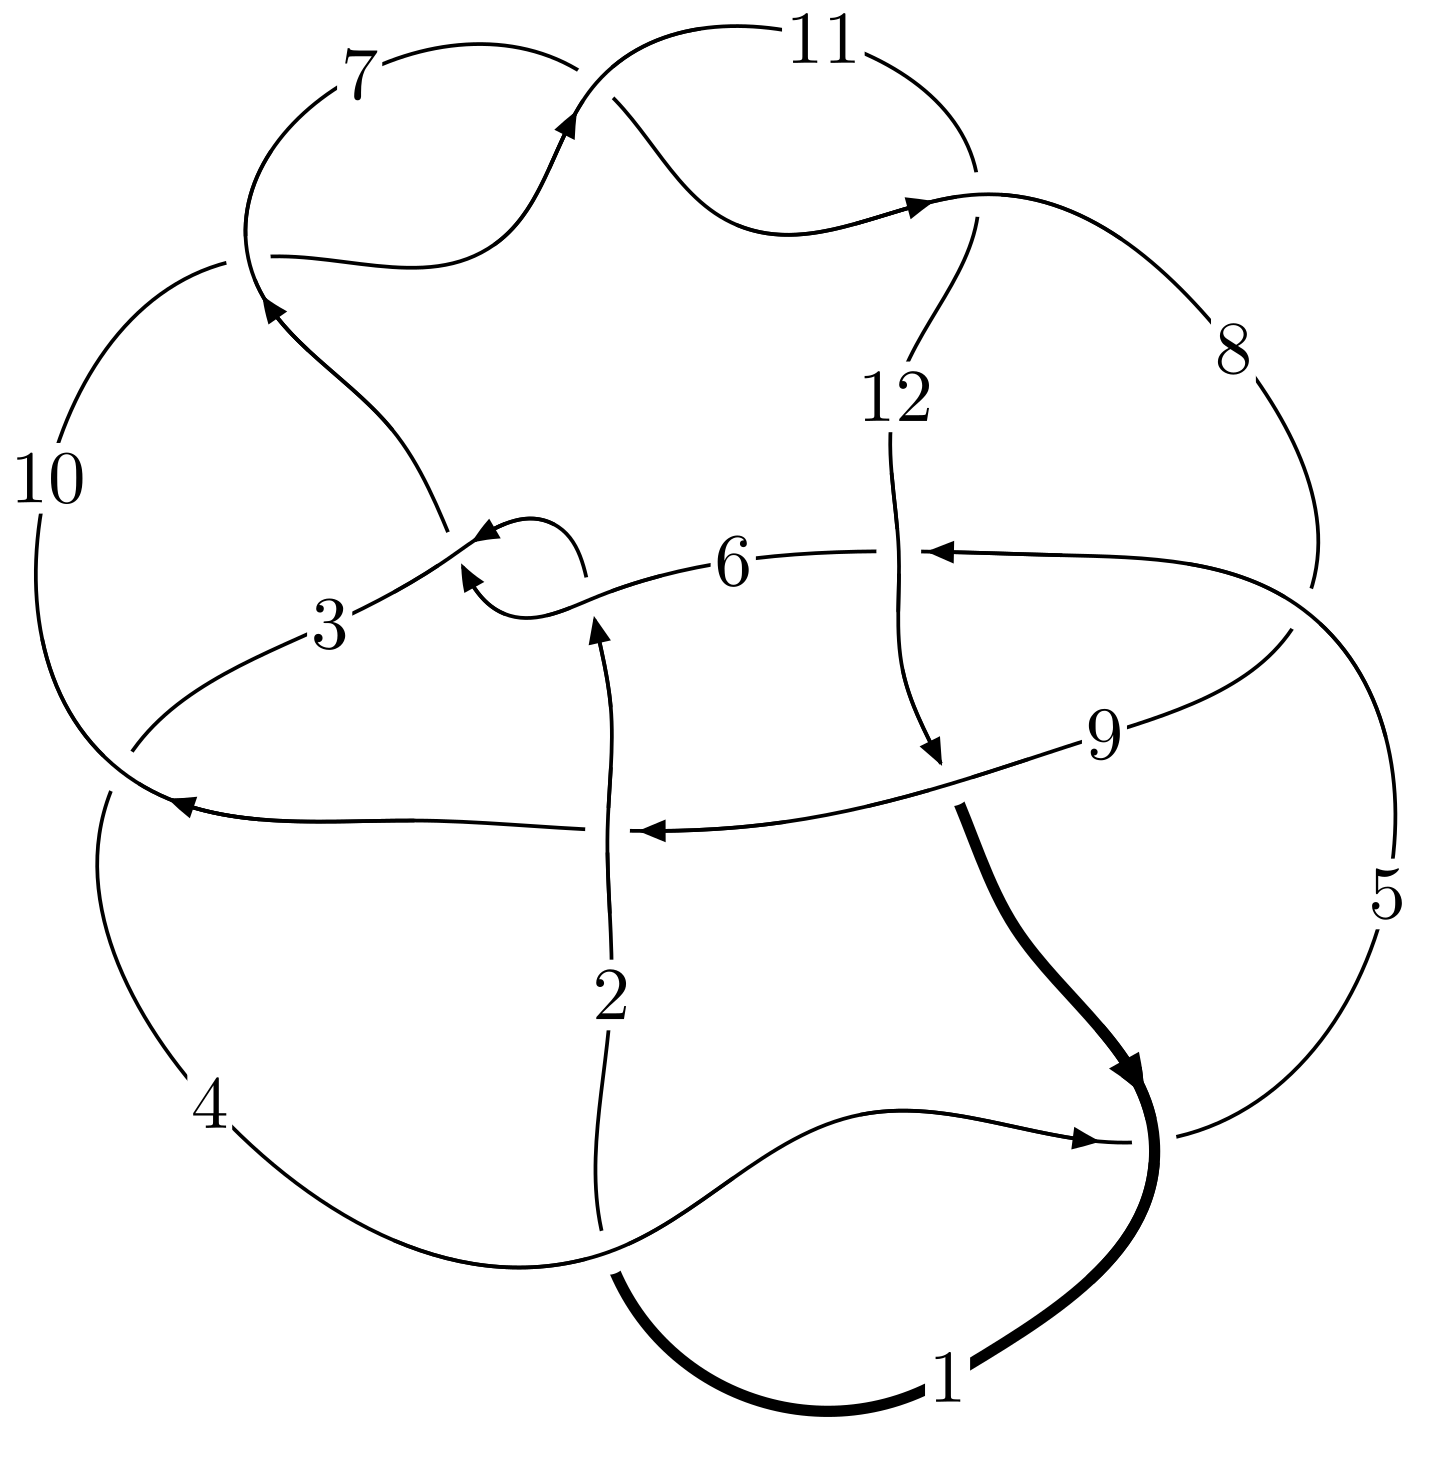
\includegraphics[width=112pt]{../../../GIT/diagram.site/Diagrams/png/1773_12a_0972.png}\\
\ \ \ A knot diagram\footnotemark}&
\allowdisplaybreaks
\textbf{Linearized knot diagam} \\
\cline{2-2}
 &
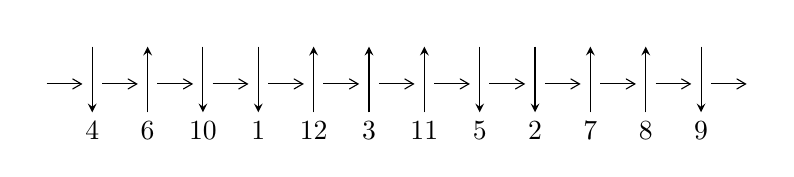
\begin{tikzpicture}[x=20pt, y=17pt]
	% nodes
	\node (C0) at (0, 0) {};
	\node (C1) at (1, 0) {};
	\node (C1U) at (1, +1) {};
	\node (C1D) at (1, -1) {4};

	\node (C2) at (2, 0) {};
	\node (C2U) at (2, +1) {};
	\node (C2D) at (2, -1) {6};

	\node (C3) at (3, 0) {};
	\node (C3U) at (3, +1) {};
	\node (C3D) at (3, -1) {10};

	\node (C4) at (4, 0) {};
	\node (C4U) at (4, +1) {};
	\node (C4D) at (4, -1) {1};

	\node (C5) at (5, 0) {};
	\node (C5U) at (5, +1) {};
	\node (C5D) at (5, -1) {12};

	\node (C6) at (6, 0) {};
	\node (C6U) at (6, +1) {};
	\node (C6D) at (6, -1) {3};

	\node (C7) at (7, 0) {};
	\node (C7U) at (7, +1) {};
	\node (C7D) at (7, -1) {11};

	\node (C8) at (8, 0) {};
	\node (C8U) at (8, +1) {};
	\node (C8D) at (8, -1) {5};

	\node (C9) at (9, 0) {};
	\node (C9U) at (9, +1) {};
	\node (C9D) at (9, -1) {2};

	\node (C10) at (10, 0) {};
	\node (C10U) at (10, +1) {};
	\node (C10D) at (10, -1) {7};

	\node (C11) at (11, 0) {};
	\node (C11U) at (11, +1) {};
	\node (C11D) at (11, -1) {8};

	\node (C12) at (12, 0) {};
	\node (C12U) at (12, +1) {};
	\node (C12D) at (12, -1) {9};
	\node (C13) at (13, 0) {};

	% arrows
	\draw[->,>={angle 60}]
	(C0) edge (C1) (C1) edge (C2) (C2) edge (C3) (C3) edge (C4) (C4) edge (C5) (C5) edge (C6) (C6) edge (C7) (C7) edge (C8) (C8) edge (C9) (C9) edge (C10) (C10) edge (C11) (C11) edge (C12) (C12) edge (C13) ;	\draw[->,>=stealth]
	(C1U) edge (C1D) (C2D) edge (C2U) (C3U) edge (C3D) (C4U) edge (C4D) (C5D) edge (C5U) (C6D) edge (C6U) (C7D) edge (C7U) (C8U) edge (C8D) (C9U) edge (C9D) (C10D) edge (C10U) (C11D) edge (C11U) (C12U) edge (C12D) ;
	\end{tikzpicture} \\
\hhline{~~} \\& 
\textbf{Solving Sequence} \\ \cline{2-2} 
 &
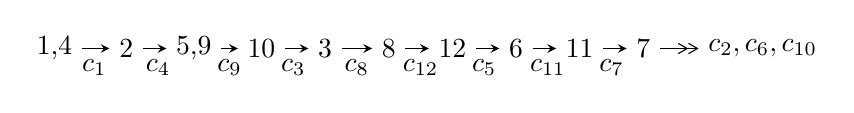
\begin{tikzpicture}[x=23pt, y=7pt]
	% node
	\node (A0) at (-1/8, 0) {1,4};
	\node (A1) at (1, 0) {2};
	\node (A2) at (33/16, 0) {5,9};
	\node (A3) at (25/8, 0) {10};
	\node (A4) at (33/8, 0) {3};
	\node (A5) at (41/8, 0) {8};
	\node (A6) at (49/8, 0) {12};
	\node (A7) at (57/8, 0) {6};
	\node (A8) at (65/8, 0) {11};
	\node (A9) at (73/8, 0) {7};
	\node (C1) at (1/2, -1) {$c_{1}$};
	\node (C2) at (3/2, -1) {$c_{4}$};
	\node (C3) at (21/8, -1) {$c_{9}$};
	\node (C4) at (29/8, -1) {$c_{3}$};
	\node (C5) at (37/8, -1) {$c_{8}$};
	\node (C6) at (45/8, -1) {$c_{12}$};
	\node (C7) at (53/8, -1) {$c_{5}$};
	\node (C8) at (61/8, -1) {$c_{11}$};
	\node (C9) at (69/8, -1) {$c_{7}$};
	\node (A10) at (11, 0) {$c_{2},c_{6},c_{10}$};

	% edge
	\draw[->,>=stealth]	
	(A0) edge (A1) (A1) edge (A2) (A2) edge (A3) (A3) edge (A4) (A4) edge (A5) (A5) edge (A6) (A6) edge (A7) (A7) edge (A8) (A8) edge (A9) ;
	\draw[->>,>={angle 60}]	
	(A9) edge (A10);
\end{tikzpicture} \\ 

\end{tabular} \\

\footnotetext{
The image of knot diagram is generated by the software ``\textbf{Draw programme}" developed by Andrew Bartholomew(\url{http://www.layer8.co.uk/maths/draw/index.htm\#Running-draw}), where we modified some parts for our purpose(\url{https://github.com/CATsTAILs/LinksPainter}).
}\phantom \\ \newline 
\centering \textbf{Ideals for irreducible components\footnotemark of $X_{\text{par}}$} 
 
\begin{align*}
I^u_{1}&=\langle 
-3.33659\times10^{517} u^{123}-2.62653\times10^{518} u^{122}+\cdots+7.25046\times10^{517} b-7.78473\times10^{519},\\
\phantom{I^u_{1}}&\phantom{= \langle  }7.51746\times10^{517} u^{123}+5.96534\times10^{518} u^{122}+\cdots+3.62523\times10^{517} a+2.21034\times10^{520},\\
\phantom{I^u_{1}}&\phantom{= \langle  }u^{124}+8 u^{123}+\cdots+1020 u+25\rangle \\
I^u_{2}&=\langle 
-56752991233 u^{24}+158661941328 u^{23}+\cdots+5813851019 b-156448380402,\\
\phantom{I^u_{2}}&\phantom{= \langle  }54545560767 u^{24}-135581602385 u^{23}+\cdots+5813851019 a+178623668066,\\
\phantom{I^u_{2}}&\phantom{= \langle  }u^{25}-3 u^{24}+\cdots+12 u-1\rangle \\
I^u_{3}&=\langle 
b+a-1,\;a^2- a u-1,\;u^2+1\rangle \\
I^u_{4}&=\langle 
b^2- b u-1,\;a+u+1,\;u^2+1\rangle \\
\\
\end{align*}
\raggedright * 4 irreducible components of $\dim_{\mathbb{C}}=0$, with total 157 representations.\\
\footnotetext{All coefficients of polynomials are rational numbers. But the coefficients are sometimes approximated in decimal forms when there is not enough margin.}
\newpage
\renewcommand{\arraystretch}{1}
\centering \section*{I. $I^u_{1}= \langle -3.34\times10^{517} u^{123}-2.63\times10^{518} u^{122}+\cdots+7.25\times10^{517} b-7.78\times10^{519},\;7.52\times10^{517} u^{123}+5.97\times10^{518} u^{122}+\cdots+3.63\times10^{517} a+2.21\times10^{520},\;u^{124}+8 u^{123}+\cdots+1020 u+25 \rangle$}
\flushleft \textbf{(i) Arc colorings}\\
\begin{tabular}{m{7pt} m{180pt} m{7pt} m{180pt} }
\flushright $a_{1}=$&$\begin{pmatrix}1\\0\end{pmatrix}$ \\
\flushright $a_{4}=$&$\begin{pmatrix}0\\u\end{pmatrix}$ \\
\flushright $a_{2}=$&$\begin{pmatrix}1\\u^2\end{pmatrix}$ \\
\flushright $a_{5}=$&$\begin{pmatrix}- u\\u\end{pmatrix}$ \\
\flushright $a_{9}=$&$\begin{pmatrix}-2.07365 u^{123}-16.4551 u^{122}+\cdots-18728.8 u-609.710\\0.460190 u^{123}+3.62257 u^{122}+\cdots+3417.67 u+107.369\end{pmatrix}$ \\
\flushright $a_{10}=$&$\begin{pmatrix}-2.55174 u^{123}-20.2391 u^{122}+\cdots-22231.5 u-720.432\\0.501200 u^{123}+3.94634 u^{122}+\cdots+3388.10 u+106.351\end{pmatrix}$ \\
\flushright $a_{3}=$&$\begin{pmatrix}-0.172222 u^{123}-1.30964 u^{122}+\cdots-2393.35 u-89.8196\\-0.0485654 u^{123}-0.490524 u^{122}+\cdots+30.4635 u+1.72975\end{pmatrix}$ \\
\flushright $a_{8}=$&$\begin{pmatrix}-2.10538 u^{123}-16.7006 u^{122}+\cdots-18765.2 u-611.590\\0.491915 u^{123}+3.86811 u^{122}+\cdots+3454.04 u+109.249\end{pmatrix}$ \\
\flushright $a_{12}=$&$\begin{pmatrix}0.204772 u^{123}+1.65803 u^{122}+\cdots+2202.56 u+63.8312\\0.111811 u^{123}+0.849694 u^{122}+\cdots+584.422 u+21.3400\end{pmatrix}$ \\
\flushright $a_{6}=$&$\begin{pmatrix}0.262764 u^{123}+2.05155 u^{122}+\cdots+2742.48 u+96.0581\\-0.0466158 u^{123}-0.277827 u^{122}+\cdots+11.3702 u+0.354091\end{pmatrix}$ \\
\flushright $a_{11}=$&$\begin{pmatrix}0.0217255 u^{123}+0.115731 u^{122}+\cdots+230.179 u+20.1115\\0.156984 u^{123}+1.22636 u^{122}+\cdots-208.931 u-7.59340\end{pmatrix}$ \\
\flushright $a_{7}=$&$\begin{pmatrix}0.0393133 u^{123}+0.404225 u^{122}+\cdots+637.111 u+11.6719\\-0.179527 u^{123}-1.42858 u^{122}+\cdots+33.3632 u+2.71980\end{pmatrix}$\\&\end{tabular}
\flushleft \textbf{(ii) Obstruction class $= -1$}\\~\\
\flushleft \textbf{(iii) Cusp Shapes $= 2.48574 u^{123}+19.4677 u^{122}+\cdots+18568.3 u+600.544$}\\~\\
\newpage\renewcommand{\arraystretch}{1}
\flushleft \textbf{(iv) u-Polynomials at the component}\newline \\
\begin{tabular}{m{50pt}|m{274pt}}
Crossings & \hspace{64pt}u-Polynomials at each crossing \\
\hline $$\begin{aligned}c_{1},c_{4}\end{aligned}$$&$\begin{aligned}
&u^{124}-8 u^{123}+\cdots-1020 u+25
\end{aligned}$\\
\hline $$\begin{aligned}c_{2},c_{6}\end{aligned}$$&$\begin{aligned}
&u^{124}-3 u^{123}+\cdots+7019 u+802
\end{aligned}$\\
\hline $$\begin{aligned}c_{3}\end{aligned}$$&$\begin{aligned}
&u^{124}+u^{123}+\cdots-323613671 u+225151331
\end{aligned}$\\
\hline $$\begin{aligned}c_{5}\end{aligned}$$&$\begin{aligned}
&u^{124}-3 u^{123}+\cdots+58197 u+6844
\end{aligned}$\\
\hline $$\begin{aligned}c_{7},c_{10},c_{11}\end{aligned}$$&$\begin{aligned}
&u^{124}-4 u^{123}+\cdots+86 u+31
\end{aligned}$\\
\hline $$\begin{aligned}c_{8}\end{aligned}$$&$\begin{aligned}
&u^{124}+4 u^{123}+\cdots-448142 u+166093
\end{aligned}$\\
\hline $$\begin{aligned}c_{9}\end{aligned}$$&$\begin{aligned}
&u^{124}+u^{123}+\cdots-308331 u+65281
\end{aligned}$\\
\hline $$\begin{aligned}c_{12}\end{aligned}$$&$\begin{aligned}
&u^{124}-4 u^{123}+\cdots-307 u+47
\end{aligned}$\\
\hline
\end{tabular}\\~\\
\newpage\renewcommand{\arraystretch}{1}
\flushleft \textbf{(v) Riley Polynomials at the component}\newline \\
\begin{tabular}{m{50pt}|m{274pt}}
Crossings & \hspace{64pt}Riley Polynomials at each crossing \\
\hline $$\begin{aligned}c_{1},c_{4}\end{aligned}$$&$\begin{aligned}
&y^{124}+102 y^{123}+\cdots-108550 y+625
\end{aligned}$\\
\hline $$\begin{aligned}c_{2},c_{6}\end{aligned}$$&$\begin{aligned}
&y^{124}-87 y^{123}+\cdots-39793137 y+643204
\end{aligned}$\\
\hline $$\begin{aligned}c_{3}\end{aligned}$$&$\begin{aligned}
&y^{124}+71 y^{123}+\cdots+2087042095852583975 y+50693121851071561
\end{aligned}$\\
\hline $$\begin{aligned}c_{5}\end{aligned}$$&$\begin{aligned}
&y^{124}-17 y^{123}+\cdots-1045038265 y+46840336
\end{aligned}$\\
\hline $$\begin{aligned}c_{7},c_{10},c_{11}\end{aligned}$$&$\begin{aligned}
&y^{124}-144 y^{123}+\cdots-148446 y+961
\end{aligned}$\\
\hline $$\begin{aligned}c_{8}\end{aligned}$$&$\begin{aligned}
&y^{124}+56 y^{123}+\cdots+1616827756682 y+27586884649
\end{aligned}$\\
\hline $$\begin{aligned}c_{9}\end{aligned}$$&$\begin{aligned}
&y^{124}+9 y^{123}+\cdots+12388959547 y+4261608961
\end{aligned}$\\
\hline $$\begin{aligned}c_{12}\end{aligned}$$&$\begin{aligned}
&y^{124}+116 y^{122}+\cdots+46939 y+2209
\end{aligned}$\\
\hline
\end{tabular}\\~\\
\newpage\flushleft \textbf{(vi) Complex Volumes and Cusp Shapes}
$$\begin{array}{c|c|c}  
\text{Solutions to }I^u_{1}& \I (\text{vol} + \sqrt{-1}CS) & \text{Cusp shape}\\
 \hline 
\begin{aligned}
u &= \phantom{-}0.624909 + 0.789700 I \\
a &= -0.853489 + 0.286122 I \\
b &= -0.642130 - 0.250578 I\end{aligned}
 & -0.78763 - 2.51768 I & \phantom{-0.000000 } 0 \\ \hline\begin{aligned}
u &= \phantom{-}0.624909 - 0.789700 I \\
a &= -0.853489 - 0.286122 I \\
b &= -0.642130 + 0.250578 I\end{aligned}
 & -0.78763 + 2.51768 I & \phantom{-0.000000 } 0 \\ \hline\begin{aligned}
u &= \phantom{-}0.349992 + 0.953649 I \\
a &= -0.271463 + 1.190640 I \\
b &= -0.180959 - 0.264370 I\end{aligned}
 & -0.22218 - 1.86679 I & \phantom{-0.000000 } 0 \\ \hline\begin{aligned}
u &= \phantom{-}0.349992 - 0.953649 I \\
a &= -0.271463 - 1.190640 I \\
b &= -0.180959 + 0.264370 I\end{aligned}
 & -0.22218 + 1.86679 I & \phantom{-0.000000 } 0 \\ \hline\begin{aligned}
u &= \phantom{-}0.038725 + 0.970476 I \\
a &= -0.88568 - 1.25933 I \\
b &= \phantom{-}0.294809 + 0.685819 I\end{aligned}
 & \phantom{-}1.67473 - 2.05855 I & \phantom{-0.000000 } 0 \\ \hline\begin{aligned}
u &= \phantom{-}0.038725 - 0.970476 I \\
a &= -0.88568 + 1.25933 I \\
b &= \phantom{-}0.294809 - 0.685819 I\end{aligned}
 & \phantom{-}1.67473 + 2.05855 I & \phantom{-0.000000 } 0 \\ \hline\begin{aligned}
u &= \phantom{-}0.657665 + 0.795735 I \\
a &= \phantom{-}1.047720 - 0.650476 I \\
b &= \phantom{-}0.636330 - 0.005582 I\end{aligned}
 & \phantom{-}4.66580 - 2.56846 I & \phantom{-0.000000 } 0 \\ \hline\begin{aligned}
u &= \phantom{-}0.657665 - 0.795735 I \\
a &= \phantom{-}1.047720 + 0.650476 I \\
b &= \phantom{-}0.636330 + 0.005582 I\end{aligned}
 & \phantom{-}4.66580 + 2.56846 I & \phantom{-0.000000 } 0 \\ \hline\begin{aligned}
u &= -0.036730 + 1.033000 I \\
a &= \phantom{-}0.160380 + 0.775791 I \\
b &= \phantom{-}1.252330 - 0.510097 I\end{aligned}
 & \phantom{-}1.55085 + 2.30574 I & \phantom{-0.000000 } 0 \\ \hline\begin{aligned}
u &= -0.036730 - 1.033000 I \\
a &= \phantom{-}0.160380 - 0.775791 I \\
b &= \phantom{-}1.252330 + 0.510097 I\end{aligned}
 & \phantom{-}1.55085 - 2.30574 I & \phantom{-0.000000 } 0\\
 \hline 
 \end{array}$$\newpage$$\begin{array}{c|c|c}  
\text{Solutions to }I^u_{1}& \I (\text{vol} + \sqrt{-1}CS) & \text{Cusp shape}\\
 \hline 
\begin{aligned}
u &= -1.011380 + 0.252588 I \\
a &= -0.0037717 - 0.0751418 I \\
b &= -0.897491 + 0.718876 I\end{aligned}
 & \phantom{-}1.62126 + 8.65715 I & \phantom{-0.000000 } 0 \\ \hline\begin{aligned}
u &= -1.011380 - 0.252588 I \\
a &= -0.0037717 + 0.0751418 I \\
b &= -0.897491 - 0.718876 I\end{aligned}
 & \phantom{-}1.62126 - 8.65715 I & \phantom{-0.000000 } 0 \\ \hline\begin{aligned}
u &= -0.246554 + 1.041700 I \\
a &= \phantom{-}0.658400 - 0.533464 I \\
b &= -1.51137 + 0.43606 I\end{aligned}
 & \phantom{-}4.55511 - 0.41818 I & \phantom{-0.000000 } 0 \\ \hline\begin{aligned}
u &= -0.246554 - 1.041700 I \\
a &= \phantom{-}0.658400 + 0.533464 I \\
b &= -1.51137 - 0.43606 I\end{aligned}
 & \phantom{-}4.55511 + 0.41818 I & \phantom{-0.000000 } 0 \\ \hline\begin{aligned}
u &= \phantom{-}0.270265 + 0.887941 I \\
a &= \phantom{-}0.71343 + 2.21385 I \\
b &= -0.546317 - 0.768353 I\end{aligned}
 & \phantom{-}6.82810 - 1.87616 I & \phantom{-0.000000 } 0 \\ \hline\begin{aligned}
u &= \phantom{-}0.270265 - 0.887941 I \\
a &= \phantom{-}0.71343 - 2.21385 I \\
b &= -0.546317 + 0.768353 I\end{aligned}
 & \phantom{-}6.82810 + 1.87616 I & \phantom{-0.000000 } 0 \\ \hline\begin{aligned}
u &= -1.071340 + 0.092162 I \\
a &= -0.208664 - 0.113413 I \\
b &= -0.170158 + 0.674017 I\end{aligned}
 & \phantom{-}3.77859 - 0.51409 I & \phantom{-0.000000 } 0 \\ \hline\begin{aligned}
u &= -1.071340 - 0.092162 I \\
a &= -0.208664 + 0.113413 I \\
b &= -0.170158 - 0.674017 I\end{aligned}
 & \phantom{-}3.77859 + 0.51409 I & \phantom{-0.000000 } 0 \\ \hline\begin{aligned}
u &= \phantom{-}1.063660 + 0.214060 I \\
a &= -0.1030460 - 0.0422966 I \\
b &= -0.736144 - 0.498925 I\end{aligned}
 & -1.84560 - 3.48872 I & \phantom{-0.000000 } 0 \\ \hline\begin{aligned}
u &= \phantom{-}1.063660 - 0.214060 I \\
a &= -0.1030460 + 0.0422966 I \\
b &= -0.736144 + 0.498925 I\end{aligned}
 & -1.84560 + 3.48872 I & \phantom{-0.000000 } 0\\
 \hline 
 \end{array}$$\newpage$$\begin{array}{c|c|c}  
\text{Solutions to }I^u_{1}& \I (\text{vol} + \sqrt{-1}CS) & \text{Cusp shape}\\
 \hline 
\begin{aligned}
u &= \phantom{-}0.200264 + 0.858804 I \\
a &= -0.199765 - 1.383860 I \\
b &= -0.307680 + 0.078714 I\end{aligned}
 & \phantom{-}2.90937 + 0.48546 I & \phantom{-0.000000 } 0 \\ \hline\begin{aligned}
u &= \phantom{-}0.200264 - 0.858804 I \\
a &= -0.199765 + 1.383860 I \\
b &= -0.307680 - 0.078714 I\end{aligned}
 & \phantom{-}2.90937 - 0.48546 I & \phantom{-0.000000 } 0 \\ \hline\begin{aligned}
u &= \phantom{-}1.013370 + 0.476653 I \\
a &= \phantom{-}0.676023 + 0.063001 I \\
b &= -0.670930 + 0.897117 I\end{aligned}
 & \phantom{-}6.99872 + 2.80339 I & \phantom{-0.000000 } 0 \\ \hline\begin{aligned}
u &= \phantom{-}1.013370 - 0.476653 I \\
a &= \phantom{-}0.676023 - 0.063001 I \\
b &= -0.670930 - 0.897117 I\end{aligned}
 & \phantom{-}6.99872 - 2.80339 I & \phantom{-0.000000 } 0 \\ \hline\begin{aligned}
u &= -0.799360 + 0.356881 I \\
a &= \phantom{-}0.806257 - 0.572661 I \\
b &= \phantom{-}0.875329 + 0.298254 I\end{aligned}
 & \phantom{-}8.64858 - 5.00143 I & \phantom{-0.000000 } 0 \\ \hline\begin{aligned}
u &= -0.799360 - 0.356881 I \\
a &= \phantom{-}0.806257 + 0.572661 I \\
b &= \phantom{-}0.875329 - 0.298254 I\end{aligned}
 & \phantom{-}8.64858 + 5.00143 I & \phantom{-0.000000 } 0 \\ \hline\begin{aligned}
u &= \phantom{-}0.266452 + 0.829127 I \\
a &= \phantom{-}1.83248 - 0.27359 I \\
b &= \phantom{-}0.678402 + 0.277204 I\end{aligned}
 & \phantom{-}2.39633 - 2.88261 I & \phantom{-0.000000 } 0 \\ \hline\begin{aligned}
u &= \phantom{-}0.266452 - 0.829127 I \\
a &= \phantom{-}1.83248 + 0.27359 I \\
b &= \phantom{-}0.678402 - 0.277204 I\end{aligned}
 & \phantom{-}2.39633 + 2.88261 I & \phantom{-0.000000 } 0 \\ \hline\begin{aligned}
u &= -0.220377 + 1.122260 I \\
a &= -0.08409 + 1.54094 I \\
b &= \phantom{-}1.10225 - 1.21547 I\end{aligned}
 & \phantom{-}2.13812 + 3.26916 I & \phantom{-0.000000 } 0 \\ \hline\begin{aligned}
u &= -0.220377 - 1.122260 I \\
a &= -0.08409 - 1.54094 I \\
b &= \phantom{-}1.10225 + 1.21547 I\end{aligned}
 & \phantom{-}2.13812 - 3.26916 I & \phantom{-0.000000 } 0\\
 \hline 
 \end{array}$$\newpage$$\begin{array}{c|c|c}  
\text{Solutions to }I^u_{1}& \I (\text{vol} + \sqrt{-1}CS) & \text{Cusp shape}\\
 \hline 
\begin{aligned}
u &= -0.033525 + 1.161790 I \\
a &= -0.319448 - 0.632001 I \\
b &= -1.307690 + 0.414071 I\end{aligned}
 & \phantom{-}7.68363 + 3.54824 I & \phantom{-0.000000 } 0 \\ \hline\begin{aligned}
u &= -0.033525 - 1.161790 I \\
a &= -0.319448 + 0.632001 I \\
b &= -1.307690 - 0.414071 I\end{aligned}
 & \phantom{-}7.68363 - 3.54824 I & \phantom{-0.000000 } 0 \\ \hline\begin{aligned}
u &= -0.609912 + 0.568440 I \\
a &= \phantom{-}1.034620 - 0.462126 I \\
b &= -0.563121 - 0.762549 I\end{aligned}
 & \phantom{-}5.17196 - 3.18037 I & \phantom{-0.000000 } 0 \\ \hline\begin{aligned}
u &= -0.609912 - 0.568440 I \\
a &= \phantom{-}1.034620 + 0.462126 I \\
b &= -0.563121 + 0.762549 I\end{aligned}
 & \phantom{-}5.17196 + 3.18037 I & \phantom{-0.000000 } 0 \\ \hline\begin{aligned}
u &= -0.029257 + 1.167110 I \\
a &= \phantom{-}0.131424 - 1.388300 I \\
b &= -0.87769 + 1.11781 I\end{aligned}
 & \phantom{-}3.66761 - 0.84831 I & \phantom{-0.000000 } 0 \\ \hline\begin{aligned}
u &= -0.029257 - 1.167110 I \\
a &= \phantom{-}0.131424 + 1.388300 I \\
b &= -0.87769 - 1.11781 I\end{aligned}
 & \phantom{-}3.66761 + 0.84831 I & \phantom{-0.000000 } 0 \\ \hline\begin{aligned}
u &= -0.438960 + 1.099790 I \\
a &= \phantom{-}0.24387 + 1.89941 I \\
b &= \phantom{-}0.482558 - 0.359313 I\end{aligned}
 & \phantom{-}10.9005 + 9.5975 I & \phantom{-0.000000 } 0 \\ \hline\begin{aligned}
u &= -0.438960 - 1.099790 I \\
a &= \phantom{-}0.24387 - 1.89941 I \\
b &= \phantom{-}0.482558 + 0.359313 I\end{aligned}
 & \phantom{-}10.9005 - 9.5975 I & \phantom{-0.000000 } 0 \\ \hline\begin{aligned}
u &= -0.349173 + 1.141460 I \\
a &= -0.19828 - 1.61269 I \\
b &= -0.99534 + 1.37906 I\end{aligned}
 & \phantom{-}7.19616 + 6.93974 I & \phantom{-0.000000 } 0 \\ \hline\begin{aligned}
u &= -0.349173 - 1.141460 I \\
a &= -0.19828 + 1.61269 I \\
b &= -0.99534 - 1.37906 I\end{aligned}
 & \phantom{-}7.19616 - 6.93974 I & \phantom{-0.000000 } 0\\
 \hline 
 \end{array}$$\newpage$$\begin{array}{c|c|c}  
\text{Solutions to }I^u_{1}& \I (\text{vol} + \sqrt{-1}CS) & \text{Cusp shape}\\
 \hline 
\begin{aligned}
u &= -1.190790 + 0.154668 I \\
a &= \phantom{-}0.371080 + 0.177841 I \\
b &= \phantom{-}0.341879 - 0.816022 I\end{aligned}
 & \phantom{-}10.80650 - 1.25200 I & \phantom{-0.000000 } 0 \\ \hline\begin{aligned}
u &= -1.190790 - 0.154668 I \\
a &= \phantom{-}0.371080 - 0.177841 I \\
b &= \phantom{-}0.341879 + 0.816022 I\end{aligned}
 & \phantom{-}10.80650 + 1.25200 I & \phantom{-0.000000 } 0 \\ \hline\begin{aligned}
u &= \phantom{-}0.780504 + 0.066163 I \\
a &= -0.128713 + 0.108564 I \\
b &= \phantom{-}0.844438 + 0.324862 I\end{aligned}
 & -1.95401 - 0.57152 I & \phantom{-0.000000 } 0 \\ \hline\begin{aligned}
u &= \phantom{-}0.780504 - 0.066163 I \\
a &= -0.128713 - 0.108564 I \\
b &= \phantom{-}0.844438 - 0.324862 I\end{aligned}
 & -1.95401 + 0.57152 I & \phantom{-0.000000 } 0 \\ \hline\begin{aligned}
u &= -0.290920 + 1.185870 I \\
a &= \phantom{-}0.31212 - 1.72148 I \\
b &= -0.253177 + 0.413757 I\end{aligned}
 & \phantom{-}4.68545 + 6.23430 I & \phantom{-0.000000 } 0 \\ \hline\begin{aligned}
u &= -0.290920 - 1.185870 I \\
a &= \phantom{-}0.31212 + 1.72148 I \\
b &= -0.253177 - 0.413757 I\end{aligned}
 & \phantom{-}4.68545 - 6.23430 I & \phantom{-0.000000 } 0 \\ \hline\begin{aligned}
u &= \phantom{-}0.690267 + 0.316922 I \\
a &= -0.995755 - 0.423093 I \\
b &= \phantom{-}0.840804 - 0.709923 I\end{aligned}
 & \phantom{-}0.16376 + 2.13777 I & \phantom{-0.000000 } 0 \\ \hline\begin{aligned}
u &= \phantom{-}0.690267 - 0.316922 I \\
a &= -0.995755 + 0.423093 I \\
b &= \phantom{-}0.840804 + 0.709923 I\end{aligned}
 & \phantom{-}0.16376 - 2.13777 I & \phantom{-0.000000 } 0 \\ \hline\begin{aligned}
u &= \phantom{-}0.395846 + 1.178580 I \\
a &= -0.16684 - 1.61000 I \\
b &= \phantom{-}1.06584 + 1.46196 I\end{aligned}
 & \phantom{-}2.91555 - 6.35209 I & \phantom{-0.000000 } 0 \\ \hline\begin{aligned}
u &= \phantom{-}0.395846 - 1.178580 I \\
a &= -0.16684 + 1.61000 I \\
b &= \phantom{-}1.06584 - 1.46196 I\end{aligned}
 & \phantom{-}2.91555 + 6.35209 I & \phantom{-0.000000 } 0\\
 \hline 
 \end{array}$$\newpage$$\begin{array}{c|c|c}  
\text{Solutions to }I^u_{1}& \I (\text{vol} + \sqrt{-1}CS) & \text{Cusp shape}\\
 \hline 
\begin{aligned}
u &= \phantom{-}0.596773 + 1.098550 I \\
a &= -0.25305 + 1.50933 I \\
b &= -0.85387 - 1.45213 I\end{aligned}
 & \phantom{-}9.03984 - 8.60000 I & \phantom{-0.000000 } 0 \\ \hline\begin{aligned}
u &= \phantom{-}0.596773 - 1.098550 I \\
a &= -0.25305 - 1.50933 I \\
b &= -0.85387 + 1.45213 I\end{aligned}
 & \phantom{-}9.03984 + 8.60000 I & \phantom{-0.000000 } 0 \\ \hline\begin{aligned}
u &= -0.060754 + 1.248950 I \\
a &= \phantom{-}0.38576 + 1.97999 I \\
b &= -0.98013 - 1.70592 I\end{aligned}
 & \phantom{-}7.48407 + 3.86950 I & \phantom{-0.000000 } 0 \\ \hline\begin{aligned}
u &= -0.060754 - 1.248950 I \\
a &= \phantom{-}0.38576 - 1.97999 I \\
b &= -0.98013 + 1.70592 I\end{aligned}
 & \phantom{-}7.48407 - 3.86950 I & \phantom{-0.000000 } 0 \\ \hline\begin{aligned}
u &= -0.002976 + 1.259540 I \\
a &= \phantom{-}0.22912 - 2.04140 I \\
b &= \phantom{-}0.59661 + 1.30966 I\end{aligned}
 & \phantom{-}7.65870 - 2.89944 I & \phantom{-0.000000 } 0 \\ \hline\begin{aligned}
u &= -0.002976 - 1.259540 I \\
a &= \phantom{-}0.22912 + 2.04140 I \\
b &= \phantom{-}0.59661 - 1.30966 I\end{aligned}
 & \phantom{-}7.65870 + 2.89944 I & \phantom{-0.000000 } 0 \\ \hline\begin{aligned}
u &= \phantom{-}0.141193 + 1.263160 I \\
a &= \phantom{-}0.81534 + 1.28478 I \\
b &= -1.55246 - 1.20153 I\end{aligned}
 & \phantom{-}5.07326 - 2.77050 I & \phantom{-0.000000 } 0 \\ \hline\begin{aligned}
u &= \phantom{-}0.141193 - 1.263160 I \\
a &= \phantom{-}0.81534 - 1.28478 I \\
b &= -1.55246 + 1.20153 I\end{aligned}
 & \phantom{-}5.07326 + 2.77050 I & \phantom{-0.000000 } 0 \\ \hline\begin{aligned}
u &= -0.148783 + 1.262330 I \\
a &= -0.57776 - 1.52603 I \\
b &= \phantom{-}1.29356 + 1.51745 I\end{aligned}
 & \phantom{-}15.0989 + 8.7503 I & \phantom{-0.000000 } 0 \\ \hline\begin{aligned}
u &= -0.148783 - 1.262330 I \\
a &= -0.57776 + 1.52603 I \\
b &= \phantom{-}1.29356 - 1.51745 I\end{aligned}
 & \phantom{-}15.0989 - 8.7503 I & \phantom{-0.000000 } 0\\
 \hline 
 \end{array}$$\newpage$$\begin{array}{c|c|c}  
\text{Solutions to }I^u_{1}& \I (\text{vol} + \sqrt{-1}CS) & \text{Cusp shape}\\
 \hline 
\begin{aligned}
u &= -0.582223 + 0.430669 I \\
a &= -0.807574 + 0.937034 I \\
b &= \phantom{-}0.795687 + 0.282579 I\end{aligned}
 & \phantom{-}0.186508 - 0.358873 I & \phantom{-0.000000 } 0 \\ \hline\begin{aligned}
u &= -0.582223 - 0.430669 I \\
a &= -0.807574 - 0.937034 I \\
b &= \phantom{-}0.795687 - 0.282579 I\end{aligned}
 & \phantom{-}0.186508 + 0.358873 I & \phantom{-0.000000 } 0 \\ \hline\begin{aligned}
u &= \phantom{-}0.081403 + 1.299880 I \\
a &= -0.51855 + 1.64065 I \\
b &= -0.785286 - 0.992413 I\end{aligned}
 & \phantom{-}15.6448 - 7.6267 I & \phantom{-0.000000 } 0 \\ \hline\begin{aligned}
u &= \phantom{-}0.081403 - 1.299880 I \\
a &= -0.51855 - 1.64065 I \\
b &= -0.785286 + 0.992413 I\end{aligned}
 & \phantom{-}15.6448 + 7.6267 I & \phantom{-0.000000 } 0 \\ \hline\begin{aligned}
u &= -1.281450 + 0.242845 I \\
a &= -0.0408311 + 0.0638631 I \\
b &= \phantom{-}0.800570 - 0.747453 I\end{aligned}
 & \phantom{-}9.7223 + 12.0177 I & \phantom{-0.000000 } 0 \\ \hline\begin{aligned}
u &= -1.281450 - 0.242845 I \\
a &= -0.0408311 - 0.0638631 I \\
b &= \phantom{-}0.800570 + 0.747453 I\end{aligned}
 & \phantom{-}9.7223 - 12.0177 I & \phantom{-0.000000 } 0 \\ \hline\begin{aligned}
u &= -0.115983 + 1.313350 I \\
a &= -0.728401 + 1.047250 I \\
b &= -0.012768 - 0.426251 I\end{aligned}
 & \phantom{-}5.94688 + 1.48446 I & \phantom{-0.000000 } 0 \\ \hline\begin{aligned}
u &= -0.115983 - 1.313350 I \\
a &= -0.728401 - 1.047250 I \\
b &= -0.012768 + 0.426251 I\end{aligned}
 & \phantom{-}5.94688 - 1.48446 I & \phantom{-0.000000 } 0 \\ \hline\begin{aligned}
u &= \phantom{-}0.066845 + 1.328250 I \\
a &= -0.222917 + 1.234220 I \\
b &= \phantom{-}0.93865 - 1.26825 I\end{aligned}
 & \phantom{-}11.16820 - 3.35347 I & \phantom{-0.000000 } 0 \\ \hline\begin{aligned}
u &= \phantom{-}0.066845 - 1.328250 I \\
a &= -0.222917 - 1.234220 I \\
b &= \phantom{-}0.93865 + 1.26825 I\end{aligned}
 & \phantom{-}11.16820 + 3.35347 I & \phantom{-0.000000 } 0\\
 \hline 
 \end{array}$$\newpage$$\begin{array}{c|c|c}  
\text{Solutions to }I^u_{1}& \I (\text{vol} + \sqrt{-1}CS) & \text{Cusp shape}\\
 \hline 
\begin{aligned}
u &= -0.604253 + 0.284274 I \\
a &= \phantom{-}0.160861 + 0.209823 I \\
b &= \phantom{-}1.024820 - 0.722652 I\end{aligned}
 & -0.03123 + 3.63182 I & \phantom{-0.000000 } 0 \\ \hline\begin{aligned}
u &= -0.604253 - 0.284274 I \\
a &= \phantom{-}0.160861 - 0.209823 I \\
b &= \phantom{-}1.024820 + 0.722652 I\end{aligned}
 & -0.03123 - 3.63182 I & \phantom{-0.000000 } 0 \\ \hline\begin{aligned}
u &= \phantom{-}1.361590 + 0.259806 I \\
a &= \phantom{-}0.134042 - 0.046505 I \\
b &= \phantom{-}0.642655 + 0.623399 I\end{aligned}
 & \phantom{-}5.07896 - 5.21597 I & \phantom{-0.000000 } 0 \\ \hline\begin{aligned}
u &= \phantom{-}1.361590 - 0.259806 I \\
a &= \phantom{-}0.134042 + 0.046505 I \\
b &= \phantom{-}0.642655 - 0.623399 I\end{aligned}
 & \phantom{-}5.07896 + 5.21597 I & \phantom{-0.000000 } 0 \\ \hline\begin{aligned}
u &= \phantom{-}0.115361 + 0.594013 I \\
a &= \phantom{-}0.183050 - 1.248340 I \\
b &= -0.617168 - 0.084784 I\end{aligned}
 & \phantom{-}2.92156 + 0.53654 I & \phantom{-0.000000 } 0 \\ \hline\begin{aligned}
u &= \phantom{-}0.115361 - 0.594013 I \\
a &= \phantom{-}0.183050 + 1.248340 I \\
b &= -0.617168 + 0.084784 I\end{aligned}
 & \phantom{-}2.92156 - 0.53654 I & \phantom{-0.000000 } 0 \\ \hline\begin{aligned}
u &= \phantom{-}0.035448 + 0.595180 I \\
a &= \phantom{-}2.31588 - 0.64381 I \\
b &= -1.57212 + 0.38454 I\end{aligned}
 & \phantom{-}2.11788 + 1.98122 I & \phantom{-0.000000 } 0 \\ \hline\begin{aligned}
u &= \phantom{-}0.035448 - 0.595180 I \\
a &= \phantom{-}2.31588 + 0.64381 I \\
b &= -1.57212 - 0.38454 I\end{aligned}
 & \phantom{-}2.11788 - 1.98122 I & \phantom{-0.000000 } 0 \\ \hline\begin{aligned}
u &= \phantom{-}0.38607 + 1.36862 I \\
a &= -0.363176 - 1.353110 I \\
b &= \phantom{-}1.04682 + 1.11374 I\end{aligned}
 & \phantom{-}2.61430 - 4.84266 I & \phantom{-0.000000 } 0 \\ \hline\begin{aligned}
u &= \phantom{-}0.38607 - 1.36862 I \\
a &= -0.363176 + 1.353110 I \\
b &= \phantom{-}1.04682 - 1.11374 I\end{aligned}
 & \phantom{-}2.61430 + 4.84266 I & \phantom{-0.000000 } 0\\
 \hline 
 \end{array}$$\newpage$$\begin{array}{c|c|c}  
\text{Solutions to }I^u_{1}& \I (\text{vol} + \sqrt{-1}CS) & \text{Cusp shape}\\
 \hline 
\begin{aligned}
u &= \phantom{-}0.292312 + 0.489399 I \\
a &= \phantom{-}0.199051 - 0.458548 I \\
b &= -1.39633 + 0.54910 I\end{aligned}
 & \phantom{-}5.76997 - 0.74612 I & \phantom{-0.000000 } 0 \\ \hline\begin{aligned}
u &= \phantom{-}0.292312 - 0.489399 I \\
a &= \phantom{-}0.199051 + 0.458548 I \\
b &= -1.39633 - 0.54910 I\end{aligned}
 & \phantom{-}5.76997 + 0.74612 I & \phantom{-0.000000 } 0 \\ \hline\begin{aligned}
u &= -0.48655 + 1.34999 I \\
a &= -0.289379 - 1.255350 I \\
b &= -0.694847 + 1.007670 I\end{aligned}
 & \phantom{-}8.26791 + 4.86057 I & \phantom{-0.000000 } 0 \\ \hline\begin{aligned}
u &= -0.48655 - 1.34999 I \\
a &= -0.289379 + 1.255350 I \\
b &= -0.694847 - 1.007670 I\end{aligned}
 & \phantom{-}8.26791 - 4.86057 I & \phantom{-0.000000 } 0 \\ \hline\begin{aligned}
u &= -0.535208 + 0.098659 I \\
a &= -0.78607 + 1.44928 I \\
b &= -0.847060 - 0.155911 I\end{aligned}
 & \phantom{-}1.50743 - 2.98404 I & \phantom{-0.000000 } 0 \\ \hline\begin{aligned}
u &= -0.535208 - 0.098659 I \\
a &= -0.78607 - 1.44928 I \\
b &= -0.847060 + 0.155911 I\end{aligned}
 & \phantom{-}1.50743 + 2.98404 I & \phantom{-0.000000 } 0 \\ \hline\begin{aligned}
u &= -0.27166 + 1.43808 I \\
a &= -0.60645 + 1.74606 I \\
b &= \phantom{-}1.25703 - 1.39510 I\end{aligned}
 & \phantom{-}5.51165 + 6.94398 I & \phantom{-0.000000 } 0 \\ \hline\begin{aligned}
u &= -0.27166 - 1.43808 I \\
a &= -0.60645 - 1.74606 I \\
b &= \phantom{-}1.25703 + 1.39510 I\end{aligned}
 & \phantom{-}5.51165 - 6.94398 I & \phantom{-0.000000 } 0 \\ \hline\begin{aligned}
u &= \phantom{-}0.43515 + 1.40233 I \\
a &= -0.136616 - 0.696627 I \\
b &= \phantom{-}0.511825 + 0.563146 I\end{aligned}
 & \phantom{-}2.33121 - 3.38566 I & \phantom{-0.000000 } 0 \\ \hline\begin{aligned}
u &= \phantom{-}0.43515 - 1.40233 I \\
a &= -0.136616 + 0.696627 I \\
b &= \phantom{-}0.511825 - 0.563146 I\end{aligned}
 & \phantom{-}2.33121 + 3.38566 I & \phantom{-0.000000 } 0\\
 \hline 
 \end{array}$$\newpage$$\begin{array}{c|c|c}  
\text{Solutions to }I^u_{1}& \I (\text{vol} + \sqrt{-1}CS) & \text{Cusp shape}\\
 \hline 
\begin{aligned}
u &= -0.53394 + 1.37569 I \\
a &= \phantom{-}0.277630 + 1.121480 I \\
b &= \phantom{-}0.344681 - 1.123800 I\end{aligned}
 & \phantom{-}7.91427 + 6.40094 I & \phantom{-0.000000 } 0 \\ \hline\begin{aligned}
u &= -0.53394 - 1.37569 I \\
a &= \phantom{-}0.277630 - 1.121480 I \\
b &= \phantom{-}0.344681 + 1.123800 I\end{aligned}
 & \phantom{-}7.91427 - 6.40094 I & \phantom{-0.000000 } 0 \\ \hline\begin{aligned}
u &= -0.68743 + 1.30596 I \\
a &= \phantom{-}0.419653 + 0.188089 I \\
b &= -0.122827 - 0.473467 I\end{aligned}
 & \phantom{-}4.33526 - 2.51765 I & \phantom{-0.000000 } 0 \\ \hline\begin{aligned}
u &= -0.68743 - 1.30596 I \\
a &= \phantom{-}0.419653 - 0.188089 I \\
b &= -0.122827 + 0.473467 I\end{aligned}
 & \phantom{-}4.33526 + 2.51765 I & \phantom{-0.000000 } 0 \\ \hline\begin{aligned}
u &= \phantom{-}0.46522 + 1.40387 I \\
a &= \phantom{-}0.134818 + 1.328190 I \\
b &= -1.09069 - 1.08181 I\end{aligned}
 & \phantom{-}3.16484 - 8.86238 I & \phantom{-0.000000 } 0 \\ \hline\begin{aligned}
u &= \phantom{-}0.46522 - 1.40387 I \\
a &= \phantom{-}0.134818 - 1.328190 I \\
b &= -1.09069 + 1.08181 I\end{aligned}
 & \phantom{-}3.16484 + 8.86238 I & \phantom{-0.000000 } 0 \\ \hline\begin{aligned}
u &= -0.43002 + 1.44348 I \\
a &= \phantom{-}0.24949 - 1.55537 I \\
b &= -1.16636 + 1.25954 I\end{aligned}
 & \phantom{-}6.9765 + 13.7973 I & \phantom{-0.000000 } 0 \\ \hline\begin{aligned}
u &= -0.43002 - 1.44348 I \\
a &= \phantom{-}0.24949 + 1.55537 I \\
b &= -1.16636 - 1.25954 I\end{aligned}
 & \phantom{-}6.9765 - 13.7973 I & \phantom{-0.000000 } 0 \\ \hline\begin{aligned}
u &= -0.101430 + 0.473608 I \\
a &= \phantom{-}2.81834 - 0.97751 I \\
b &= -0.288841 - 0.487196 I\end{aligned}
 & \phantom{-}5.59899 - 3.09249 I & \phantom{-}8.90713 + 0. I\phantom{ +0.000000I} \\ \hline\begin{aligned}
u &= -0.101430 - 0.473608 I \\
a &= \phantom{-}2.81834 + 0.97751 I \\
b &= -0.288841 + 0.487196 I\end{aligned}
 & \phantom{-}5.59899 + 3.09249 I & \phantom{-}8.90713 + 0. I\phantom{ +0.000000I}\\
 \hline 
 \end{array}$$\newpage$$\begin{array}{c|c|c}  
\text{Solutions to }I^u_{1}& \I (\text{vol} + \sqrt{-1}CS) & \text{Cusp shape}\\
 \hline 
\begin{aligned}
u &= -0.49838 + 1.43173 I \\
a &= \phantom{-}0.301067 + 1.199040 I \\
b &= \phantom{-}0.889618 - 0.943728 I\end{aligned}
 & \phantom{-}15.8333 + 4.5792 I & \phantom{-0.000000 } 0 \\ \hline\begin{aligned}
u &= -0.49838 - 1.43173 I \\
a &= \phantom{-}0.301067 - 1.199040 I \\
b &= \phantom{-}0.889618 + 0.943728 I\end{aligned}
 & \phantom{-}15.8333 - 4.5792 I & \phantom{-0.000000 } 0 \\ \hline\begin{aligned}
u &= -0.14267 + 1.52286 I \\
a &= -0.425047 - 0.509529 I \\
b &= \phantom{-}1.112710 + 0.556637 I\end{aligned}
 & \phantom{-}15.0819 - 1.6516 I & \phantom{-0.000000 } 0 \\ \hline\begin{aligned}
u &= -0.14267 - 1.52286 I \\
a &= -0.425047 + 0.509529 I \\
b &= \phantom{-}1.112710 - 0.556637 I\end{aligned}
 & \phantom{-}15.0819 + 1.6516 I & \phantom{-0.000000 } 0 \\ \hline\begin{aligned}
u &= \phantom{-}0.51929 + 1.48104 I \\
a &= -0.036046 - 1.242720 I \\
b &= \phantom{-}1.12719 + 1.06290 I\end{aligned}
 & \phantom{-}10.5364 - 11.5662 I & \phantom{-0.000000 } 0 \\ \hline\begin{aligned}
u &= \phantom{-}0.51929 - 1.48104 I \\
a &= -0.036046 + 1.242720 I \\
b &= \phantom{-}1.12719 - 1.06290 I\end{aligned}
 & \phantom{-}10.5364 + 11.5662 I & \phantom{-0.000000 } 0 \\ \hline\begin{aligned}
u &= -0.61500 + 1.44586 I \\
a &= -0.304008 - 0.973397 I \\
b &= -0.179648 + 1.242880 I\end{aligned}
 & \phantom{-}14.9283 + 7.9258 I & \phantom{-0.000000 } 0 \\ \hline\begin{aligned}
u &= -0.61500 - 1.44586 I \\
a &= -0.304008 + 0.973397 I \\
b &= -0.179648 - 1.242880 I\end{aligned}
 & \phantom{-}14.9283 - 7.9258 I & \phantom{-0.000000 } 0 \\ \hline\begin{aligned}
u &= -0.52705 + 1.48373 I \\
a &= -0.11920 + 1.42093 I \\
b &= \phantom{-}1.15290 - 1.23181 I\end{aligned}
 & \phantom{-}15.1210 + 18.2859 I & \phantom{-0.000000 } 0 \\ \hline\begin{aligned}
u &= -0.52705 - 1.48373 I \\
a &= -0.11920 - 1.42093 I \\
b &= \phantom{-}1.15290 + 1.23181 I\end{aligned}
 & \phantom{-}15.1210 - 18.2859 I & \phantom{-0.000000 } 0\\
 \hline 
 \end{array}$$\newpage$$\begin{array}{c|c|c}  
\text{Solutions to }I^u_{1}& \I (\text{vol} + \sqrt{-1}CS) & \text{Cusp shape}\\
 \hline 
\begin{aligned}
u &= -0.03557 + 1.59893 I \\
a &= \phantom{-}1.48233 - 0.63793 I \\
b &= -1.90550 + 0.62040 I\end{aligned}
 & \phantom{-}13.09920 - 1.07183 I & \phantom{-0.000000 } 0 \\ \hline\begin{aligned}
u &= -0.03557 - 1.59893 I \\
a &= \phantom{-}1.48233 + 0.63793 I \\
b &= -1.90550 - 0.62040 I\end{aligned}
 & \phantom{-}13.09920 + 1.07183 I & \phantom{-0.000000 } 0 \\ \hline\begin{aligned}
u &= \phantom{-}0.07284 + 1.62369 I \\
a &= \phantom{-}0.350406 - 0.365184 I \\
b &= \phantom{-}0.301197 + 0.400851 I\end{aligned}
 & \phantom{-}14.8060 - 1.2582 I & \phantom{-0.000000 } 0 \\ \hline\begin{aligned}
u &= \phantom{-}0.07284 - 1.62369 I \\
a &= \phantom{-}0.350406 + 0.365184 I \\
b &= \phantom{-}0.301197 - 0.400851 I\end{aligned}
 & \phantom{-}14.8060 + 1.2582 I & \phantom{-0.000000 } 0 \\ \hline\begin{aligned}
u &= \phantom{-}0.43257 + 1.58022 I \\
a &= \phantom{-}0.148827 + 0.857592 I \\
b &= -0.609393 - 1.016200 I\end{aligned}
 & \phantom{-}10.49490 - 2.70483 I & \phantom{-0.000000 } 0 \\ \hline\begin{aligned}
u &= \phantom{-}0.43257 - 1.58022 I \\
a &= \phantom{-}0.148827 - 0.857592 I \\
b &= -0.609393 + 1.016200 I\end{aligned}
 & \phantom{-}10.49490 + 2.70483 I & \phantom{-0.000000 } 0 \\ \hline\begin{aligned}
u &= -0.144359 + 0.217920 I \\
a &= -1.32019 + 2.13894 I \\
b &= \phantom{-}0.190926 + 0.455290 I\end{aligned}
 & \phantom{-}0.095467 - 1.146130 I & \phantom{-}1.33446 + 5.20853 I \\ \hline\begin{aligned}
u &= -0.144359 - 0.217920 I \\
a &= -1.32019 - 2.13894 I \\
b &= \phantom{-}0.190926 - 0.455290 I\end{aligned}
 & \phantom{-}0.095467 + 1.146130 I & \phantom{-}1.33446 - 5.20853 I \\ \hline\begin{aligned}
u &= -0.137483 + 0.053618 I \\
a &= \phantom{-}1.88691 + 9.62828 I \\
b &= \phantom{-}0.174139 - 1.062900 I\end{aligned}
 & \phantom{-}11.29770 - 7.33389 I & \phantom{-}7.61770 + 3.62503 I \\ \hline\begin{aligned}
u &= -0.137483 - 0.053618 I \\
a &= \phantom{-}1.88691 - 9.62828 I \\
b &= \phantom{-}0.174139 + 1.062900 I\end{aligned}
 & \phantom{-}11.29770 + 7.33389 I & \phantom{-}7.61770 - 3.62503 I\\
 \hline 
 \end{array}$$\newpage$$\begin{array}{c|c|c}  
\text{Solutions to }I^u_{1}& \I (\text{vol} + \sqrt{-1}CS) & \text{Cusp shape}\\
 \hline 
\begin{aligned}
u &= -0.1074230 + 0.0204538 I \\
a &= -2.29690 - 7.62971 I \\
b &= -0.195075 + 1.214220 I\end{aligned}
 & \phantom{-}3.75165 - 3.18681 I & \phantom{-}7.79230 + 9.47115 I \\ \hline\begin{aligned}
u &= -0.1074230 - 0.0204538 I \\
a &= -2.29690 + 7.62971 I \\
b &= -0.195075 - 1.214220 I\end{aligned}
 & \phantom{-}3.75165 + 3.18681 I & \phantom{-}7.79230 - 9.47115 I \\ \hline\begin{aligned}
u &= -0.97511 + 1.97865 I \\
a &= -0.129208 - 0.152014 I \\
b &= -0.085980 + 0.379628 I\end{aligned}
 & \phantom{-}13.44110 - 3.50918 I & \phantom{-0.000000 } 0 \\ \hline\begin{aligned}
u &= -0.97511 - 1.97865 I \\
a &= -0.129208 + 0.152014 I \\
b &= -0.085980 - 0.379628 I\end{aligned}
 & \phantom{-}13.44110 + 3.50918 I & \phantom{-0.000000 } 0\\
 \hline 
 \end{array}$$\newpage\newpage\renewcommand{\arraystretch}{1}
\centering \section*{II. $I^u_{2}= \langle -5.68\times10^{10} u^{24}+1.59\times10^{11} u^{23}+\cdots+5.81\times10^{9} b-1.56\times10^{11},\;5.45\times10^{10} u^{24}-1.36\times10^{11} u^{23}+\cdots+5.81\times10^{9} a+1.79\times10^{11},\;u^{25}-3 u^{24}+\cdots+12 u-1 \rangle$}
\flushleft \textbf{(i) Arc colorings}\\
\begin{tabular}{m{7pt} m{180pt} m{7pt} m{180pt} }
\flushright $a_{1}=$&$\begin{pmatrix}1\\0\end{pmatrix}$ \\
\flushright $a_{4}=$&$\begin{pmatrix}0\\u\end{pmatrix}$ \\
\flushright $a_{2}=$&$\begin{pmatrix}1\\u^2\end{pmatrix}$ \\
\flushright $a_{5}=$&$\begin{pmatrix}- u\\u\end{pmatrix}$ \\
\flushright $a_{9}=$&$\begin{pmatrix}-9.38200 u^{24}+23.3204 u^{23}+\cdots+257.610 u-30.7238\\9.76169 u^{24}-27.2903 u^{23}+\cdots-260.709 u+26.9096\end{pmatrix}$ \\
\flushright $a_{10}=$&$\begin{pmatrix}-22.5428 u^{24}+58.9665 u^{23}+\cdots+566.844 u-62.4590\\10.0858 u^{24}-26.6485 u^{23}+\cdots-227.833 u+23.0732\end{pmatrix}$ \\
\flushright $a_{3}=$&$\begin{pmatrix}15.1635 u^{24}-34.1351 u^{23}+\cdots-227.440 u+26.2036\\0.0247429 u^{24}-3.38012 u^{23}+\cdots-75.5561 u+6.67925\end{pmatrix}$ \\
\flushright $a_{8}=$&$\begin{pmatrix}-13.3618 u^{24}+32.6426 u^{23}+\cdots+291.960 u-33.5546\\13.7415 u^{24}-36.6125 u^{23}+\cdots-295.059 u+29.7404\end{pmatrix}$ \\
\flushright $a_{12}=$&$\begin{pmatrix}3.58211 u^{24}-3.74055 u^{23}+\cdots+28.9720 u+1.80463\\8.82286 u^{24}-20.9033 u^{23}+\cdots-79.4184 u+3.70537\end{pmatrix}$ \\
\flushright $a_{6}=$&$\begin{pmatrix}24.1743 u^{24}-52.5145 u^{23}+\cdots-215.662 u+20.1633\\4.38131 u^{24}-13.2049 u^{23}+\cdots-127.203 u+11.3084\end{pmatrix}$ \\
\flushright $a_{11}=$&$\begin{pmatrix}6.89964 u^{24}-2.83690 u^{23}+\cdots+285.884 u-32.9364\\3.55480 u^{24}-7.84830 u^{23}+\cdots-73.5124 u+7.87747\end{pmatrix}$ \\
\flushright $a_{7}=$&$\begin{pmatrix}7.45497 u^{24}-6.18940 u^{23}+\cdots+259.080 u-33.2308\\2.81610 u^{24}-5.60481 u^{23}+\cdots-34.7801 u+3.55480\end{pmatrix}$\\&\end{tabular}
\flushleft \textbf{(ii) Obstruction class $= 1$}\\~\\
\flushleft \textbf{(iii) Cusp Shapes $= \frac{38880606157}{5813851019} u^{24}-\frac{204299857999}{5813851019} u^{23}+\cdots-\frac{5343011314076}{5813851019} u+\frac{647995598087}{5813851019}$}\\~\\
\newpage\renewcommand{\arraystretch}{1}
\flushleft \textbf{(iv) u-Polynomials at the component}\newline \\
\begin{tabular}{m{50pt}|m{274pt}}
Crossings & \hspace{64pt}u-Polynomials at each crossing \\
\hline $$\begin{aligned}c_{1}\end{aligned}$$&$\begin{aligned}
&u^{25}-3 u^{24}+\cdots+12 u-1
\end{aligned}$\\
\hline $$\begin{aligned}c_{2}\end{aligned}$$&$\begin{aligned}
&u^{25}+2 u^{24}+\cdots- u+1
\end{aligned}$\\
\hline $$\begin{aligned}c_{3}\end{aligned}$$&$\begin{aligned}
&u^{25}+2 u^{23}+\cdots- u-1
\end{aligned}$\\
\hline $$\begin{aligned}c_{4}\end{aligned}$$&$\begin{aligned}
&u^{25}+3 u^{24}+\cdots+12 u+1
\end{aligned}$\\
\hline $$\begin{aligned}c_{5}\end{aligned}$$&$\begin{aligned}
&u^{25}+4 u^{24}+\cdots- u+1
\end{aligned}$\\
\hline $$\begin{aligned}c_{6}\end{aligned}$$&$\begin{aligned}
&u^{25}-2 u^{24}+\cdots- u-1
\end{aligned}$\\
\hline $$\begin{aligned}c_{7}\end{aligned}$$&$\begin{aligned}
&u^{25}-5 u^{24}+\cdots+2 u+1
\end{aligned}$\\
\hline $$\begin{aligned}c_{8}\end{aligned}$$&$\begin{aligned}
&u^{25}- u^{24}+\cdots+5 u^2+1
\end{aligned}$\\
\hline $$\begin{aligned}c_{9}\end{aligned}$$&$\begin{aligned}
&u^{25}-2 u^{23}+\cdots+u+1
\end{aligned}$\\
\hline $$\begin{aligned}c_{10},c_{11}\end{aligned}$$&$\begin{aligned}
&u^{25}+5 u^{24}+\cdots+2 u-1
\end{aligned}$\\
\hline $$\begin{aligned}c_{12}\end{aligned}$$&$\begin{aligned}
&u^{25}-5 u^{24}+\cdots+u-1
\end{aligned}$\\
\hline
\end{tabular}\\~\\
\newpage\renewcommand{\arraystretch}{1}
\flushleft \textbf{(v) Riley Polynomials at the component}\newline \\
\begin{tabular}{m{50pt}|m{274pt}}
Crossings & \hspace{64pt}Riley Polynomials at each crossing \\
\hline $$\begin{aligned}c_{1},c_{4}\end{aligned}$$&$\begin{aligned}
&y^{25}+23 y^{24}+\cdots+12 y-1
\end{aligned}$\\
\hline $$\begin{aligned}c_{2},c_{6}\end{aligned}$$&$\begin{aligned}
&y^{25}-14 y^{24}+\cdots+19 y-1
\end{aligned}$\\
\hline $$\begin{aligned}c_{3}\end{aligned}$$&$\begin{aligned}
&y^{25}+4 y^{24}+\cdots-41 y-1
\end{aligned}$\\
\hline $$\begin{aligned}c_{5}\end{aligned}$$&$\begin{aligned}
&y^{25}+30 y^{23}+\cdots+y-1
\end{aligned}$\\
\hline $$\begin{aligned}c_{7},c_{10},c_{11}\end{aligned}$$&$\begin{aligned}
&y^{25}-35 y^{24}+\cdots-20 y-1
\end{aligned}$\\
\hline $$\begin{aligned}c_{8}\end{aligned}$$&$\begin{aligned}
&y^{25}+11 y^{24}+\cdots-10 y-1
\end{aligned}$\\
\hline $$\begin{aligned}c_{9}\end{aligned}$$&$\begin{aligned}
&y^{25}-4 y^{24}+\cdots+y-1
\end{aligned}$\\
\hline $$\begin{aligned}c_{12}\end{aligned}$$&$\begin{aligned}
&y^{25}-3 y^{24}+\cdots+11 y-1
\end{aligned}$\\
\hline
\end{tabular}\\~\\
\newpage\flushleft \textbf{(vi) Complex Volumes and Cusp Shapes}
$$\begin{array}{c|c|c}  
\text{Solutions to }I^u_{2}& \I (\text{vol} + \sqrt{-1}CS) & \text{Cusp shape}\\
 \hline 
\begin{aligned}
u &= \phantom{-}0.396533 + 0.918439 I \\
a &= \phantom{-}0.246592 - 0.656324 I \\
b &= \phantom{-}0.801411 + 0.091216 I\end{aligned}
 & \phantom{-}2.78380 - 1.71389 I & \phantom{-}1.54455 + 2.94870 I \\ \hline\begin{aligned}
u &= \phantom{-}0.396533 - 0.918439 I \\
a &= \phantom{-}0.246592 + 0.656324 I \\
b &= \phantom{-}0.801411 - 0.091216 I\end{aligned}
 & \phantom{-}2.78380 + 1.71389 I & \phantom{-}1.54455 - 2.94870 I \\ \hline\begin{aligned}
u &= -0.522963 + 0.749559 I \\
a &= -0.254600 + 0.036431 I \\
b &= \phantom{-}0.416621 - 0.514156 I\end{aligned}
 & \phantom{-}3.86969 - 1.94885 I & \phantom{-}6.67029 + 1.25514 I \\ \hline\begin{aligned}
u &= -0.522963 - 0.749559 I \\
a &= -0.254600 - 0.036431 I \\
b &= \phantom{-}0.416621 + 0.514156 I\end{aligned}
 & \phantom{-}3.86969 + 1.94885 I & \phantom{-}6.67029 - 1.25514 I \\ \hline\begin{aligned}
u &= \phantom{-}0.599632 + 0.688427 I \\
a &= -0.990660 + 0.161060 I \\
b &= -0.660665 - 0.309143 I\end{aligned}
 & -0.80491 - 2.72003 I & -1.4684 + 21.3189 I \\ \hline\begin{aligned}
u &= \phantom{-}0.599632 - 0.688427 I \\
a &= -0.990660 - 0.161060 I \\
b &= -0.660665 + 0.309143 I\end{aligned}
 & -0.80491 + 2.72003 I & -1.4684 - 21.3189 I \\ \hline\begin{aligned}
u &= -0.454087 + 1.030360 I \\
a &= \phantom{-}1.03190 + 1.63681 I \\
b &= \phantom{-}0.113347 - 0.973124 I\end{aligned}
 & \phantom{-}12.0422 + 9.0646 I & \phantom{-}9.38473 - 6.78978 I \\ \hline\begin{aligned}
u &= -0.454087 - 1.030360 I \\
a &= \phantom{-}1.03190 - 1.63681 I \\
b &= \phantom{-}0.113347 + 0.973124 I\end{aligned}
 & \phantom{-}12.0422 - 9.0646 I & \phantom{-}9.38473 + 6.78978 I \\ \hline\begin{aligned}
u &= \phantom{-}0.673443 + 0.377672 I \\
a &= -1.022940 - 0.727811 I \\
b &= \phantom{-}0.797515 - 0.772015 I\end{aligned}
 & \phantom{-}4.43310 + 3.33564 I & -0.43428 - 4.34078 I \\ \hline\begin{aligned}
u &= \phantom{-}0.673443 - 0.377672 I \\
a &= -1.022940 + 0.727811 I \\
b &= \phantom{-}0.797515 + 0.772015 I\end{aligned}
 & \phantom{-}4.43310 - 3.33564 I & -0.43428 + 4.34078 I\\
 \hline 
 \end{array}$$\newpage$$\begin{array}{c|c|c}  
\text{Solutions to }I^u_{2}& \I (\text{vol} + \sqrt{-1}CS) & \text{Cusp shape}\\
 \hline 
\begin{aligned}
u &= \phantom{-}0.445519 + 1.181260 I \\
a &= \phantom{-}0.11767 - 1.61358 I \\
b &= \phantom{-}0.98415 + 1.46104 I\end{aligned}
 & \phantom{-}6.96031 - 7.72852 I & \phantom{-}4.03159 + 8.91256 I \\ \hline\begin{aligned}
u &= \phantom{-}0.445519 - 1.181260 I \\
a &= \phantom{-}0.11767 + 1.61358 I \\
b &= \phantom{-}0.98415 - 1.46104 I\end{aligned}
 & \phantom{-}6.96031 + 7.72852 I & \phantom{-}4.03159 - 8.91256 I \\ \hline\begin{aligned}
u &= \phantom{-}0.528550 + 0.447594 I \\
a &= \phantom{-}1.84401 + 0.70055 I \\
b &= \phantom{-}0.634465 + 0.380510 I\end{aligned}
 & \phantom{-}4.87746 - 3.64656 I & \phantom{-}1.63258 + 6.77129 I \\ \hline\begin{aligned}
u &= \phantom{-}0.528550 - 0.447594 I \\
a &= \phantom{-}1.84401 - 0.70055 I \\
b &= \phantom{-}0.634465 - 0.380510 I\end{aligned}
 & \phantom{-}4.87746 + 3.64656 I & \phantom{-}1.63258 - 6.77129 I \\ \hline\begin{aligned}
u &= -0.318652 + 1.283850 I \\
a &= -0.13770 - 1.74819 I \\
b &= -0.442802 + 1.266680 I\end{aligned}
 & \phantom{-}6.26588 + 5.52732 I & \phantom{-}6.98548 - 5.31379 I \\ \hline\begin{aligned}
u &= -0.318652 - 1.283850 I \\
a &= -0.13770 + 1.74819 I \\
b &= -0.442802 - 1.266680 I\end{aligned}
 & \phantom{-}6.26588 - 5.52732 I & \phantom{-}6.98548 + 5.31379 I \\ \hline\begin{aligned}
u &= \phantom{-}0.350396 + 1.325240 I \\
a &= \phantom{-}0.41285 + 1.48160 I \\
b &= -1.15583 - 1.30583 I\end{aligned}
 & \phantom{-}3.29730 - 5.21881 I & \phantom{-}8.57149 + 5.00846 I \\ \hline\begin{aligned}
u &= \phantom{-}0.350396 - 1.325240 I \\
a &= \phantom{-}0.41285 - 1.48160 I \\
b &= -1.15583 + 1.30583 I\end{aligned}
 & \phantom{-}3.29730 + 5.21881 I & \phantom{-}8.57149 - 5.00846 I \\ \hline\begin{aligned}
u &= \phantom{-}0.424493 + 0.266239 I \\
a &= \phantom{-}1.44747 + 0.85701 I \\
b &= -0.981579 + 0.594218 I\end{aligned}
 & -0.42081 + 1.85133 I & -5.86069 - 1.68765 I \\ \hline\begin{aligned}
u &= \phantom{-}0.424493 - 0.266239 I \\
a &= \phantom{-}1.44747 - 0.85701 I \\
b &= -0.981579 - 0.594218 I\end{aligned}
 & -0.42081 - 1.85133 I & -5.86069 + 1.68765 I\\
 \hline 
 \end{array}$$\newpage$$\begin{array}{c|c|c}  
\text{Solutions to }I^u_{2}& \I (\text{vol} + \sqrt{-1}CS) & \text{Cusp shape}\\
 \hline 
\begin{aligned}
u &= -0.01425 + 1.64121 I \\
a &= -1.286330 + 0.308438 I \\
b &= \phantom{-}1.69344 - 0.22865 I\end{aligned}
 & \phantom{-}12.91170 - 0.79888 I & \phantom{-}3.16117 - 8.46251 I \\ \hline\begin{aligned}
u &= -0.01425 - 1.64121 I \\
a &= -1.286330 - 0.308438 I \\
b &= \phantom{-}1.69344 + 0.22865 I\end{aligned}
 & \phantom{-}12.91170 + 0.79888 I & \phantom{-}3.16117 + 8.46251 I \\ \hline\begin{aligned}
u &= \phantom{-}0.270555\phantom{ +0.000000I} \\
a &= -2.92223\phantom{ +0.000000I} \\
b &= \phantom{-}1.20005\phantom{ +0.000000I}\end{aligned}
 & \phantom{-}5.82532\phantom{ +0.000000I} & \phantom{-}8.15020\phantom{ +0.000000I} \\ \hline\begin{aligned}
u &= -0.74389 + 1.89057 I \\
a &= \phantom{-}0.0528490 + 0.0450918 I \\
b &= -0.300101 + 0.199881 I\end{aligned}
 & \phantom{-}13.24880 - 3.52025 I & \phantom{-0.000000 } 0 \\ \hline\begin{aligned}
u &= -0.74389 - 1.89057 I \\
a &= \phantom{-}0.0528490 - 0.0450918 I \\
b &= -0.300101 - 0.199881 I\end{aligned}
 & \phantom{-}13.24880 + 3.52025 I & \phantom{-0.000000 } 0\\
 \hline 
 \end{array}$$\newpage\newpage\renewcommand{\arraystretch}{1}
\centering \section*{III. $I^u_{3}= \langle b+a-1,\;a^2- a u-1,\;u^2+1 \rangle$}
\flushleft \textbf{(i) Arc colorings}\\
\begin{tabular}{m{7pt} m{180pt} m{7pt} m{180pt} }
\flushright $a_{1}=$&$\begin{pmatrix}1\\0\end{pmatrix}$ \\
\flushright $a_{4}=$&$\begin{pmatrix}0\\u\end{pmatrix}$ \\
\flushright $a_{2}=$&$\begin{pmatrix}1\\-1\end{pmatrix}$ \\
\flushright $a_{5}=$&$\begin{pmatrix}- u\\u\end{pmatrix}$ \\
\flushright $a_{9}=$&$\begin{pmatrix}a\\- a+1\end{pmatrix}$ \\
\flushright $a_{10}=$&$\begin{pmatrix}a-1\\- a+2\end{pmatrix}$ \\
\flushright $a_{3}=$&$\begin{pmatrix}-2 a u- a+2 u\\3 a u+a-2 u\end{pmatrix}$ \\
\flushright $a_{8}=$&$\begin{pmatrix}a-1\\- a+2\end{pmatrix}$ \\
\flushright $a_{12}=$&$\begin{pmatrix}a u- a+2\\- a u+2 a-2\end{pmatrix}$ \\
\flushright $a_{6}=$&$\begin{pmatrix}a u+a-2 u-1\\- a u-2 a+3 u+1\end{pmatrix}$ \\
\flushright $a_{11}=$&$\begin{pmatrix}a u+1\\- a u+a\end{pmatrix}$ \\
\flushright $a_{7}=$&$\begin{pmatrix}- a u+a-2\\a u-2 a+2\end{pmatrix}$\\&\end{tabular}
\flushleft \textbf{(ii) Obstruction class $= 1$}\\~\\
\flushleft \textbf{(iii) Cusp Shapes $= 4 a u+8$}\\~\\
\newpage\renewcommand{\arraystretch}{1}
\flushleft \textbf{(iv) u-Polynomials at the component}\newline \\
\begin{tabular}{m{50pt}|m{274pt}}
Crossings & \hspace{64pt}u-Polynomials at each crossing \\
\hline $$\begin{aligned}c_{1},c_{4},c_{8}\end{aligned}$$&$\begin{aligned}
&(u^2+1)^2
\end{aligned}$\\
\hline $$\begin{aligned}c_{2},c_{6}\end{aligned}$$&$\begin{aligned}
&u^4- u^2+1
\end{aligned}$\\
\hline $$\begin{aligned}c_{3}\end{aligned}$$&$\begin{aligned}
&u^4-2 u^3+5 u^2-4 u+1
\end{aligned}$\\
\hline $$\begin{aligned}c_{5}\end{aligned}$$&$\begin{aligned}
&(u^2- u+1)^2
\end{aligned}$\\
\hline $$\begin{aligned}c_{7},c_{9}\end{aligned}$$&$\begin{aligned}
&(u+1)^4
\end{aligned}$\\
\hline $$\begin{aligned}c_{10},c_{11}\end{aligned}$$&$\begin{aligned}
&(u-1)^4
\end{aligned}$\\
\hline $$\begin{aligned}c_{12}\end{aligned}$$&$\begin{aligned}
&u^4-4 u^3+5 u^2-2 u+1
\end{aligned}$\\
\hline
\end{tabular}\\~\\
\newpage\renewcommand{\arraystretch}{1}
\flushleft \textbf{(v) Riley Polynomials at the component}\newline \\
\begin{tabular}{m{50pt}|m{274pt}}
Crossings & \hspace{64pt}Riley Polynomials at each crossing \\
\hline $$\begin{aligned}c_{1},c_{4},c_{8}\end{aligned}$$&$\begin{aligned}
&(y+1)^4
\end{aligned}$\\
\hline $$\begin{aligned}c_{2},c_{6}\end{aligned}$$&$\begin{aligned}
&(y^2- y+1)^2
\end{aligned}$\\
\hline $$\begin{aligned}c_{3}\end{aligned}$$&$\begin{aligned}
&y^4+6 y^3+11 y^2-6 y+1
\end{aligned}$\\
\hline $$\begin{aligned}c_{5}\end{aligned}$$&$\begin{aligned}
&(y^2+y+1)^2
\end{aligned}$\\
\hline $$\begin{aligned}c_{7},c_{9},c_{10}\\c_{11}\end{aligned}$$&$\begin{aligned}
&(y-1)^4
\end{aligned}$\\
\hline $$\begin{aligned}c_{12}\end{aligned}$$&$\begin{aligned}
&y^4-6 y^3+11 y^2+6 y+1
\end{aligned}$\\
\hline
\end{tabular}\\~\\
\newpage\flushleft \textbf{(vi) Complex Volumes and Cusp Shapes}
$$\begin{array}{c|c|c}  
\text{Solutions to }I^u_{3}& \I (\text{vol} + \sqrt{-1}CS) & \text{Cusp shape}\\
 \hline 
\begin{aligned}
u &= \phantom{-0.000000 -}1.000000 I \\
a &= -0.866025 + 0.500000 I \\
b &= \phantom{-}1.86603 - 0.50000 I\end{aligned}
 & \phantom{-}3.28987 - 2.02988 I & \phantom{-}6.00000 + 3.46410 I \\ \hline\begin{aligned}
u &= \phantom{-0.000000 -}1.000000 I \\
a &= \phantom{-}0.866025 + 0.500000 I \\
b &= \phantom{-}0.133975 - 0.500000 I\end{aligned}
 & \phantom{-}3.28987 + 2.02988 I & \phantom{-}6.00000 - 3.46410 I \\ \hline\begin{aligned}
u &= \phantom{-0.000000 } -1.000000 I \\
a &= -0.866025 - 0.500000 I \\
b &= \phantom{-}1.86603 + 0.50000 I\end{aligned}
 & \phantom{-}3.28987 + 2.02988 I & \phantom{-}6.00000 - 3.46410 I \\ \hline\begin{aligned}
u &= \phantom{-0.000000 } -1.000000 I \\
a &= \phantom{-}0.866025 - 0.500000 I \\
b &= \phantom{-}0.133975 + 0.500000 I\end{aligned}
 & \phantom{-}3.28987 - 2.02988 I & \phantom{-}6.00000 + 3.46410 I\\
 \hline 
 \end{array}$$\newpage\newpage\renewcommand{\arraystretch}{1}
\centering \section*{IV. $I^u_{4}= \langle b^2- b u-1,\;a+u+1,\;u^2+1 \rangle$}
\flushleft \textbf{(i) Arc colorings}\\
\begin{tabular}{m{7pt} m{180pt} m{7pt} m{180pt} }
\flushright $a_{1}=$&$\begin{pmatrix}1\\0\end{pmatrix}$ \\
\flushright $a_{4}=$&$\begin{pmatrix}0\\u\end{pmatrix}$ \\
\flushright $a_{2}=$&$\begin{pmatrix}1\\-1\end{pmatrix}$ \\
\flushright $a_{5}=$&$\begin{pmatrix}- u\\u\end{pmatrix}$ \\
\flushright $a_{9}=$&$\begin{pmatrix}- u-1\\b\end{pmatrix}$ \\
\flushright $a_{10}=$&$\begin{pmatrix}- b\\2 b- u-1\end{pmatrix}$ \\
\flushright $a_{3}=$&$\begin{pmatrix}- b+u\\b u+b- u\end{pmatrix}$ \\
\flushright $a_{8}=$&$\begin{pmatrix}- b\\2 b- u-1\end{pmatrix}$ \\
\flushright $a_{12}=$&$\begin{pmatrix}b u+b+1\\- b u-1\end{pmatrix}$ \\
\flushright $a_{6}=$&$\begin{pmatrix}- b-1\\u+1\end{pmatrix}$ \\
\flushright $a_{11}=$&$\begin{pmatrix}b u+1\\- b u+2 b- u-2\end{pmatrix}$ \\
\flushright $a_{7}=$&$\begin{pmatrix}- b u- b-1\\b u+1\end{pmatrix}$\\&\end{tabular}
\flushleft \textbf{(ii) Obstruction class $= 1$}\\~\\
\flushleft \textbf{(iii) Cusp Shapes $= 4 b u+8$}\\~\\
\newpage\renewcommand{\arraystretch}{1}
\flushleft \textbf{(iv) u-Polynomials at the component}\newline \\
\begin{tabular}{m{50pt}|m{274pt}}
Crossings & \hspace{64pt}u-Polynomials at each crossing \\
\hline $$\begin{aligned}c_{1},c_{4}\end{aligned}$$&$\begin{aligned}
&(u^2+1)^2
\end{aligned}$\\
\hline $$\begin{aligned}c_{2},c_{6},c_{12}\end{aligned}$$&$\begin{aligned}
&u^4- u^2+1
\end{aligned}$\\
\hline $$\begin{aligned}c_{3}\end{aligned}$$&$\begin{aligned}
&(u^2+u+1)^2
\end{aligned}$\\
\hline $$\begin{aligned}c_{5}\end{aligned}$$&$\begin{aligned}
&(u^2- u+1)^2
\end{aligned}$\\
\hline $$\begin{aligned}c_{7}\end{aligned}$$&$\begin{aligned}
&(u+1)^4
\end{aligned}$\\
\hline $$\begin{aligned}c_{8}\end{aligned}$$&$\begin{aligned}
&u^4-2 u^3+5 u^2-4 u+1
\end{aligned}$\\
\hline $$\begin{aligned}c_{9}\end{aligned}$$&$\begin{aligned}
&u^4-4 u^3+5 u^2-2 u+1
\end{aligned}$\\
\hline $$\begin{aligned}c_{10},c_{11}\end{aligned}$$&$\begin{aligned}
&(u-1)^4
\end{aligned}$\\
\hline
\end{tabular}\\~\\
\newpage\renewcommand{\arraystretch}{1}
\flushleft \textbf{(v) Riley Polynomials at the component}\newline \\
\begin{tabular}{m{50pt}|m{274pt}}
Crossings & \hspace{64pt}Riley Polynomials at each crossing \\
\hline $$\begin{aligned}c_{1},c_{4}\end{aligned}$$&$\begin{aligned}
&(y+1)^4
\end{aligned}$\\
\hline $$\begin{aligned}c_{2},c_{6},c_{12}\end{aligned}$$&$\begin{aligned}
&(y^2- y+1)^2
\end{aligned}$\\
\hline $$\begin{aligned}c_{3},c_{5}\end{aligned}$$&$\begin{aligned}
&(y^2+y+1)^2
\end{aligned}$\\
\hline $$\begin{aligned}c_{7},c_{10},c_{11}\end{aligned}$$&$\begin{aligned}
&(y-1)^4
\end{aligned}$\\
\hline $$\begin{aligned}c_{8}\end{aligned}$$&$\begin{aligned}
&y^4+6 y^3+11 y^2-6 y+1
\end{aligned}$\\
\hline $$\begin{aligned}c_{9}\end{aligned}$$&$\begin{aligned}
&y^4-6 y^3+11 y^2+6 y+1
\end{aligned}$\\
\hline
\end{tabular}\\~\\
\newpage\flushleft \textbf{(vi) Complex Volumes and Cusp Shapes}
$$\begin{array}{c|c|c}  
\text{Solutions to }I^u_{4}& \I (\text{vol} + \sqrt{-1}CS) & \text{Cusp shape}\\
 \hline 
\begin{aligned}
u &= \phantom{-0.000000 -}1.000000 I \\
a &= -1.00000 - 1.00000 I \\
b &= -0.866025 + 0.500000 I\end{aligned}
 & \phantom{-}3.28987 - 2.02988 I & \phantom{-}6.00000 + 3.46410 I \\ \hline\begin{aligned}
u &= \phantom{-0.000000 -}1.000000 I \\
a &= -1.00000 - 1.00000 I \\
b &= \phantom{-}0.866025 + 0.500000 I\end{aligned}
 & \phantom{-}3.28987 + 2.02988 I & \phantom{-}6.00000 - 3.46410 I \\ \hline\begin{aligned}
u &= \phantom{-0.000000 } -1.000000 I \\
a &= -1.00000 + 1.00000 I \\
b &= -0.866025 - 0.500000 I\end{aligned}
 & \phantom{-}3.28987 + 2.02988 I & \phantom{-}6.00000 - 3.46410 I \\ \hline\begin{aligned}
u &= \phantom{-0.000000 } -1.000000 I \\
a &= -1.00000 + 1.00000 I \\
b &= \phantom{-}0.866025 - 0.500000 I\end{aligned}
 & \phantom{-}3.28987 - 2.02988 I & \phantom{-}6.00000 + 3.46410 I\\
 \hline 
 \end{array}$$\newpage
\newpage\renewcommand{\arraystretch}{1}
\centering \section*{ V. u-Polynomials}
\begin{tabular}{m{50pt}|m{274pt}}
Crossings & \hspace{64pt}u-Polynomials at each crossing \\
\hline $$\begin{aligned}c_{1}\end{aligned}$$&$\begin{aligned}
&((u^2+1)^4)(u^{25}-3 u^{24}+\cdots+12 u-1)(u^{124}-8 u^{123}+\cdots-1020 u+25)
\end{aligned}$\\
\hline $$\begin{aligned}c_{2}\end{aligned}$$&$\begin{aligned}
&((u^4- u^2+1)^2)(u^{25}+2 u^{24}+\cdots- u+1)\\
&\cdot(u^{124}-3 u^{123}+\cdots+7019 u+802)
\end{aligned}$\\
\hline $$\begin{aligned}c_{3}\end{aligned}$$&$\begin{aligned}
&((u^2+u+1)^2)(u^4-2 u^3+\cdots-4 u+1)(u^{25}+2 u^{23}+\cdots- u-1)\\
&\cdot(u^{124}+u^{123}+\cdots-323613671 u+225151331)
\end{aligned}$\\
\hline $$\begin{aligned}c_{4}\end{aligned}$$&$\begin{aligned}
&((u^2+1)^4)(u^{25}+3 u^{24}+\cdots+12 u+1)(u^{124}-8 u^{123}+\cdots-1020 u+25)
\end{aligned}$\\
\hline $$\begin{aligned}c_{5}\end{aligned}$$&$\begin{aligned}
&((u^2- u+1)^4)(u^{25}+4 u^{24}+\cdots- u+1)\\
&\cdot(u^{124}-3 u^{123}+\cdots+58197 u+6844)
\end{aligned}$\\
\hline $$\begin{aligned}c_{6}\end{aligned}$$&$\begin{aligned}
&((u^4- u^2+1)^2)(u^{25}-2 u^{24}+\cdots- u-1)\\
&\cdot(u^{124}-3 u^{123}+\cdots+7019 u+802)
\end{aligned}$\\
\hline $$\begin{aligned}c_{7}\end{aligned}$$&$\begin{aligned}
&((u+1)^8)(u^{25}-5 u^{24}+\cdots+2 u+1)(u^{124}-4 u^{123}+\cdots+86 u+31)
\end{aligned}$\\
\hline $$\begin{aligned}c_{8}\end{aligned}$$&$\begin{aligned}
&((u^2+1)^2)(u^4-2 u^3+\cdots-4 u+1)(u^{25}- u^{24}+\cdots+5 u^2+1)\\
&\cdot(u^{124}+4 u^{123}+\cdots-448142 u+166093)
\end{aligned}$\\
\hline $$\begin{aligned}c_{9}\end{aligned}$$&$\begin{aligned}
&((u+1)^4)(u^4-4 u^3+\cdots-2 u+1)(u^{25}-2 u^{23}+\cdots+u+1)\\
&\cdot(u^{124}+u^{123}+\cdots-308331 u+65281)
\end{aligned}$\\
\hline $$\begin{aligned}c_{10},c_{11}\end{aligned}$$&$\begin{aligned}
&((u-1)^8)(u^{25}+5 u^{24}+\cdots+2 u-1)(u^{124}-4 u^{123}+\cdots+86 u+31)
\end{aligned}$\\
\hline $$\begin{aligned}c_{12}\end{aligned}$$&$\begin{aligned}
&(u^4- u^2+1)(u^4-4 u^3+\cdots-2 u+1)(u^{25}-5 u^{24}+\cdots+u-1)\\
&\cdot(u^{124}-4 u^{123}+\cdots-307 u+47)
\end{aligned}$\\
\hline
\end{tabular}\newpage\renewcommand{\arraystretch}{1}
\centering \section*{ VI. Riley Polynomials}
\begin{tabular}{m{50pt}|m{274pt}}
Crossings & \hspace{64pt}Riley Polynomials at each crossing \\
\hline $$\begin{aligned}c_{1},c_{4}\end{aligned}$$&$\begin{aligned}
&((y+1)^8)(y^{25}+23 y^{24}+\cdots+12 y-1)\\
&\cdot(y^{124}+102 y^{123}+\cdots-108550 y+625)
\end{aligned}$\\
\hline $$\begin{aligned}c_{2},c_{6}\end{aligned}$$&$\begin{aligned}
&((y^2- y+1)^4)(y^{25}-14 y^{24}+\cdots+19 y-1)\\
&\cdot(y^{124}-87 y^{123}+\cdots-39793137 y+643204)
\end{aligned}$\\
\hline $$\begin{aligned}c_{3}\end{aligned}$$&$\begin{aligned}
&((y^2+y+1)^2)(y^4+6 y^3+\cdots-6 y+1)(y^{25}+4 y^{24}+\cdots-41 y-1)\\
&\cdot(y^{124}+71 y^{123}+\cdots+2087042095852583975 y+50693121851071561)
\end{aligned}$\\
\hline $$\begin{aligned}c_{5}\end{aligned}$$&$\begin{aligned}
&((y^2+y+1)^4)(y^{25}+30 y^{23}+\cdots+y-1)\\
&\cdot(y^{124}-17 y^{123}+\cdots-1045038265 y+46840336)
\end{aligned}$\\
\hline $$\begin{aligned}c_{7},c_{10},c_{11}\end{aligned}$$&$\begin{aligned}
&((y-1)^8)(y^{25}-35 y^{24}+\cdots-20 y-1)\\
&\cdot(y^{124}-144 y^{123}+\cdots-148446 y+961)
\end{aligned}$\\
\hline $$\begin{aligned}c_{8}\end{aligned}$$&$\begin{aligned}
&((y+1)^4)(y^4+6 y^3+\cdots-6 y+1)(y^{25}+11 y^{24}+\cdots-10 y-1)\\
&\cdot(y^{124}+56 y^{123}+\cdots+1616827756682 y+27586884649)
\end{aligned}$\\
\hline $$\begin{aligned}c_{9}\end{aligned}$$&$\begin{aligned}
&((y-1)^4)(y^4-6 y^3+\cdots+6 y+1)(y^{25}-4 y^{24}+\cdots+y-1)\\
&\cdot(y^{124}+9 y^{123}+\cdots+12388959547 y+4261608961)
\end{aligned}$\\
\hline $$\begin{aligned}c_{12}\end{aligned}$$&$\begin{aligned}
&((y^2- y+1)^2)(y^4-6 y^3+\cdots+6 y+1)(y^{25}-3 y^{24}+\cdots+11 y-1)\\
&\cdot(y^{124}+116 y^{122}+\cdots+46939 y+2209)
\end{aligned}$\\
\hline
\end{tabular}
\vskip 2pc
\end{document}